\centering
\begin{blackbox}{Textual Representation}
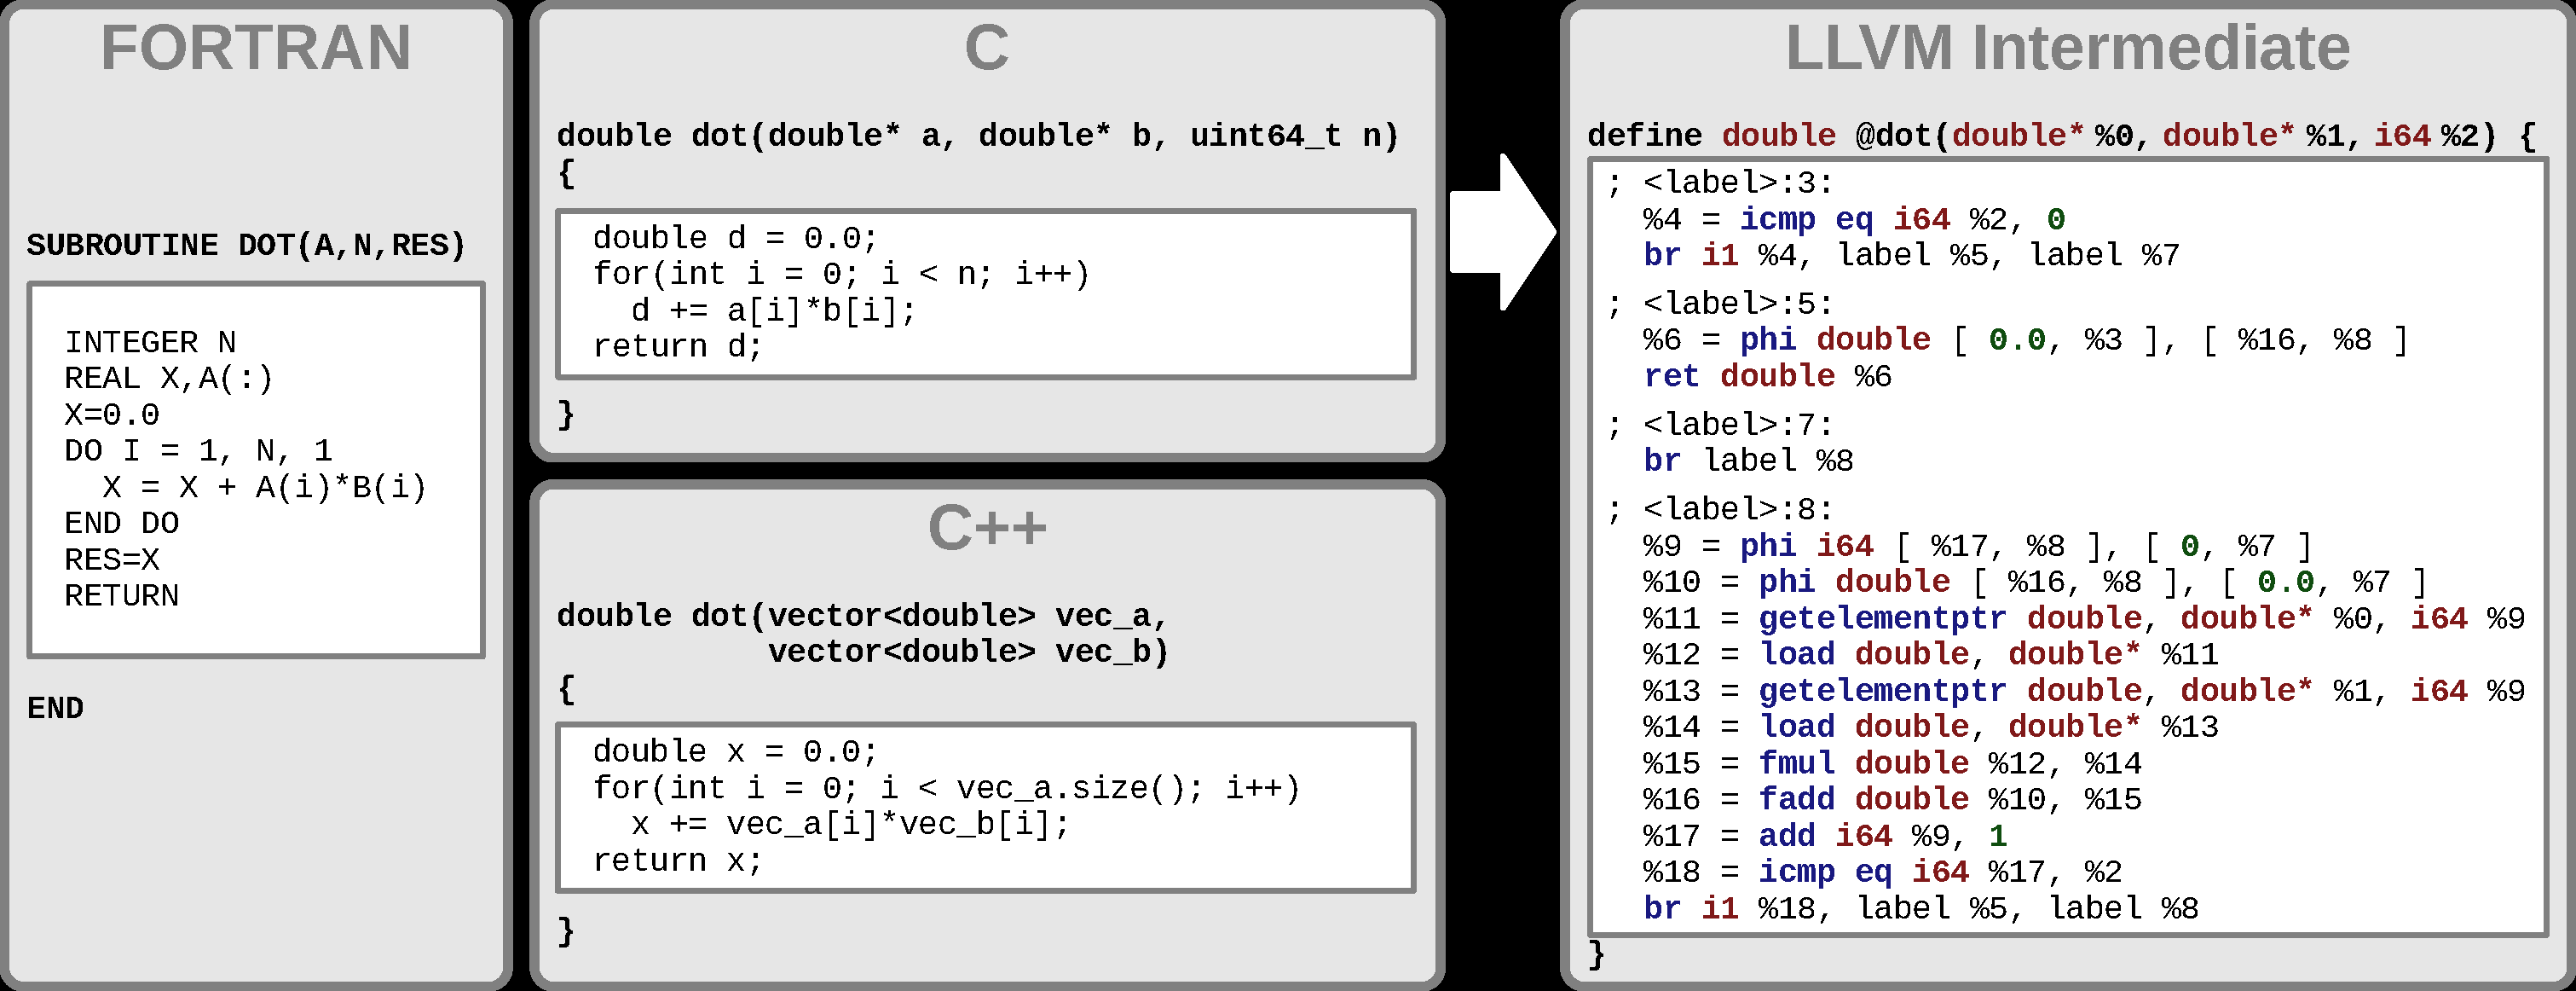
\includegraphics[width=\columnwidth]{figures/model_representations_textual}
\end{blackbox}


\includegraphics[width=\columnwidth]{figures/model_arrows_upper}

\begin{blackbox}{Structural Representation}
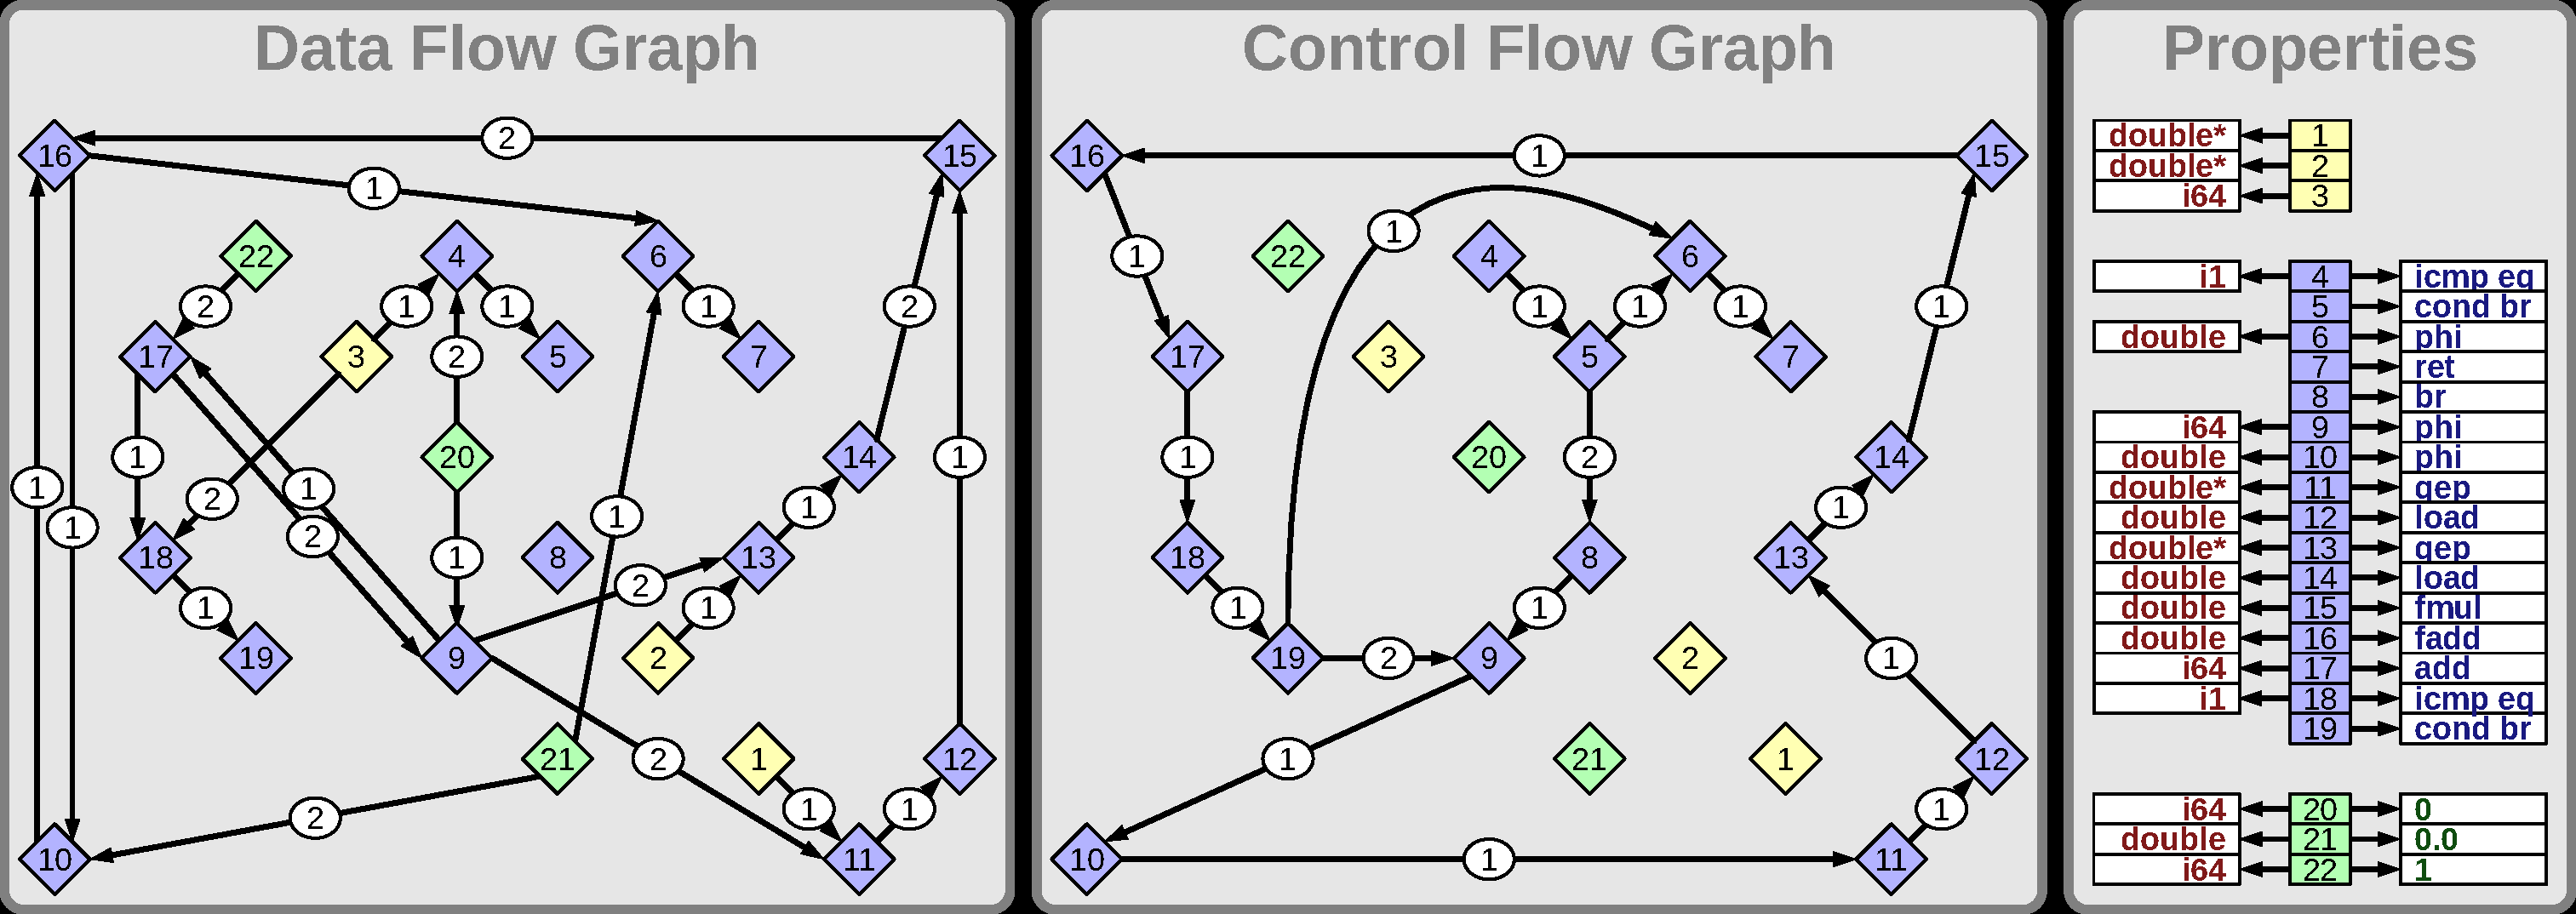
\includegraphics[width=\columnwidth]{figures/model_representations_structure}
\end{blackbox}


\includegraphics[width=\columnwidth]{figures/model_arrows_lower}

\begin{blackbox}{Mathematical Representation}
    \centering
    \begin{minipage}{0.329\textwidth}
        \begin{graybox}
            \scriptsize
            \setlength{\abovedisplayskip}{0pt}
            \setlength{\belowdisplayskip}{0pt}
            \vspace{-0.5em}
            \begin{align*}
                DF&G_\mathcal F=\{(1,1,11),(1,2,13)\\[-0.5em]
                  &(1,3,4),(2,3,18),(1,4,5),\\[-0.5em]
                  &(1,6,7),(2,9,11),(2,9,13),\\[-0.5em]
                  &(1,9,17),(1,10,16),(1,11,12),\\[-0.5em]
                  &(1,12,15),(1,13,14),(2,14,15),\\[-0.5em]
                  &(2,15,16),(2,16,6),(2,16,10),\\[-0.5em]
                  &(2,17,9),(1,17,18),(1,18,19),\\[-0.5em]
                  &(2,20,4),(1,20,9),(1,21,6),\\[-0.5em]
                  &(1,21,10),(2,22,17)\}\subset\mathbb N^3
            \end{align*}
        \end{graybox}
    \end{minipage}
    \begin{minipage}{0.329\textwidth}
        \begin{graybox}
            \scriptsize
            \setlength{\abovedisplayskip}{0pt}
            \setlength{\belowdisplayskip}{0pt}
            \vspace{-0.5em}
            \begin{align*}
                CFG_\mathcal F=\{&(1,4,5),(1,5,6),\\[-0.5em]
                  &(2,5,8),(1,6,7),\\[-0.5em]
                  &(1,8,9),(1,9,10),\\[-0.5em]
                  &(1,10,11),(1,11,12),\\[-0.5em]
                  &(1,12,13),(1,13,14),\\[-0.5em]
                  &(1,14,15),(1,15,16),\\[-0.5em]
                  &(1,16,17),(1,17,18),\\[-0.5em]
                  &(1,18,19),(1,19,6),\\[-0.5em]
                  &(2,19,9)\}\subset\mathbb N^3
            \end{align*}
        \end{graybox}
    \end{minipage}
    \begin{minipage}{0.329\textwidth}
        \centering
        \begin{graybox}
            \scriptsize
            \setlength{\abovedisplayskip}{0pt}
            \setlength{\belowdisplayskip}{0pt}
            \vspace{-0.5em}
            \begin{align*}
                T_\mathcal F={}&\{(\textit{double*},1),(\textit{double*},2),\dots\}\\[-0.5em]
                      \subset{}&Types_\text{LLVM}\times\mathbb N\\[-0.25em]
                P_\mathcal F={}&\{1,2,3\}\subset\mathbb N\\[-0.25em]
                I_\mathcal F={}&\{(\textit{icmp eq},4),(\textit{cond br},5),\dots\}\\[-0.5em]
                      \subset{}&Opcodes_\text{LLVM}\times\mathbb N\\[-0.25em]
                G_\mathcal F={}&\{\}\subset GlobalNames_\text{LLVM}\times\mathbb N\\[-0.25em]
                C_\mathcal F={}&\{(0,20),(0,21),(1,22)\}\\[-0.5em]
                      \subset{}&\mathbb R\times\mathbb N
            \end{align*}

            \vspace{0.45em}
        \end{graybox}
    \end{minipage}

    \begin{minipage}{0.55\textwidth}
        \begin{graybox}
            \setlength{\abovedisplayskip}{0pt}
            \setlength{\belowdisplayskip}{0pt}
            \vspace{-0.5em}
            \begin{align*}
                M_{dot}=(DFG_\mathcal{F},
                 CFG_\mathcal{F},
                 T_\mathcal{F},
                 P_\mathcal{F},
                 I_\mathcal{F},
                 G_\mathcal{F},
                 C_\mathcal{F})
            \end{align*}
        \end{graybox}
    \end{minipage}
\end{blackbox}